\chapter[Cas applicatif et prérequis]{Cas applicatif et prérequis} \label{C2}

\boitemagique{Dans ce chapitre}{
Nous présentons les travaux prérequis pour nos expérimentations présentées dans les chapitres 3 et 4. Nous développons le contexte applicatif servant d'illustration au travers d'un cas d'usage. Un point sera fait sur la création des jeux de données. Puis nous verrons la génération d'explications locales. Enfin les interfaces de visualisation seront énumérées.
}

% Intro
Dans ce chapitre, nous définissons le contexte applicatif sur lequel nous menons nos expérimentations. Les prérequis tels que la création et collecte des données sont passés en revue. Nous générons des explications locales pour les experts du domaine, et proposons différentes visualisations d'explications.

% Objectif du chapitre
Ce chapitre présente ainsi tous les prérequis nécessaires à la réalisation des expérimentations présentées dans les chapitres 3 et 4. Les matériaux présentés font appel à la labellisation manuelle de données, à la génération d'explications vues dans la littérature, mais aussi à la création d'un démonstrateur et la préparation des visualisations à y intégrer.
% on en retirera quoi ?
Nous discuterons des problématiques rencontrées, telles que la définition d'une vérité terrain, et les avantages et inconvénients des méthodes de génération d'explications utilisées.

% Plan
La première section est consacrée à la présentation du cas d'usage et des données associées, dont une partie est labellisée manuellement. La seconde section présente la génération des explications. Enfin, en section~\ref{C2:demonstrateur}, nous détaillons l'implémentation des différentes visualisations dans un démonstrateur.

\section{Présentation du contexte LEGO} \label{C2:usecase}

Nous abordons l'explicabilité des modèles profonds dans le cadre spécifique du traitement de la langue naturelle. Afin de définir et appréhender ce contexte, nous illustrons nos travaux avec un cas d'usage de traitement de textes.

Un cas d'usage de Pôle emploi est le tri automatique des offres non conformes. Ce cas d'usage est appelé \textit{LEGO}, pour LEGalité des Offres. Pôle emploi publie mensuellement 250 000 offres internes et maintient un stock d'environ 600 000 offres partenaires, agrégées de sites tels que Monster ou Jobijoba. Ces offres passent par un processus de vérification avant d'être publiées; afin de répondre aux critères de qualité. À ce jour, il existe plus de 70 motifs de non-conformité. Parmi eux, le dépassement d'un nombre maximal de caractères et les champs manquants sont vérifiés automatiquement avec succès. Reste la vérification des points plus difficiles à détecter tels que les discriminations sur les candidats (âge) ou encore des points contractuels (``CDD pouvant évoluer vers un CDI'').

Ce processus de vérification a longtemps été effectué par un système à base d'expressions régulières, formant un ensemble complexe de règles aux effets de bord inattendus. Ce système historique a été un premier pas vers l’automatisation. Toutefois, il a produit des erreurs que nous retrouvons dans les données les plus anciennes.

La DSI de Pôle emploi a automatisé le tri des offres non conformes, via un système composé de plusieurs modèles d'analyse sémantique. Ce système actuel lève des alertes non contraignantes pour les agents de Pôle emploi, et des refus contraignants pour les recruteurs et recruteuses. Donner au personnel les raisons des alertes de leurs offres permet l'harmonisation des bonnes pratiques. Pour les recruteurs, l'intérêt est double : leur permettre de corriger leur offre et donc de publier sur le site, et réduire leur frustration liée au rejet.

La figure~\ref{fig:ihm_DUNE} présente l'interface de travail des conseillers et conseillères à dominante entreprise (CDE) pour la création d'une offre d'emploi. L'alerte est présente sur un bandeau jaune en haut de page, en surlignant le champ incriminé ``Descriptif de poste'' et en affichant la phrase problématique et l'alerte associée : ``Droit du travail : Type de poste''.  L'alerte est remontée grâce à l'outil de tri automatique des offres non conformes.

\begin{figure}[htpb!]
    \centering
    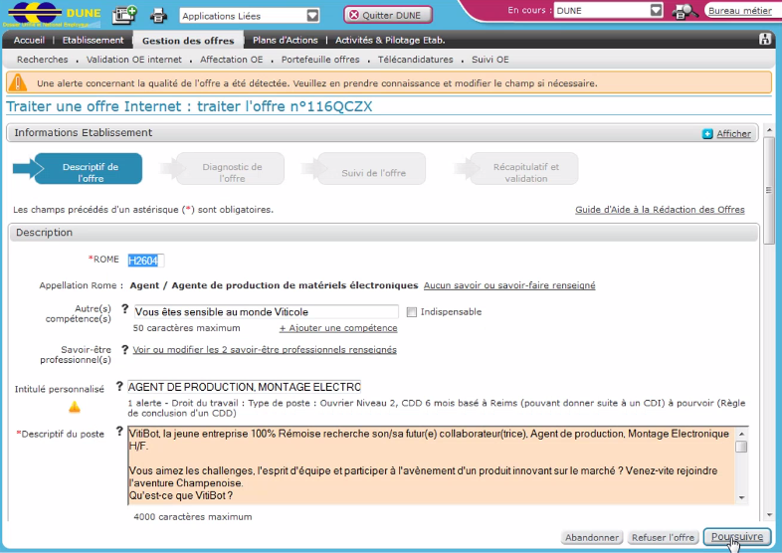
\includegraphics[width=0.9\textwidth]{S2-Explicabilite_locale/figures/Dune.png}
    \caption{Interface de l'outil de création d'offre avec une alerte liée au contrat de travail. L'alerte est accompagnée de la phrase incriminée. Le champ concerné, ``Descriptif de poste'', est surligné en jaune pour attirer l'attention de l'utilisateur. Iel peut ignorer l'alerte et cliquer sur le bouton ``poursuivre''.}
    \label{fig:ihm_DUNE}
\end{figure}

Le système actuel se concentre sur l’analyse sémantique des phrases des offres, afin de détecter un sous ensemble de motifs de non-conformité. La détection se fait au niveau des phrases d'offres d'emploi, sur le respect ou non des critères de conformité, avec 27 motifs possibles, dont le motif ``vide'' correspondant aux offres légales. Nous avons ainsi un problème de classification multi-classes. Le cas multi-label, soit le cas où une même phrase possède plusieurs motifs de rejets, correspond à moins de $1\%$ des cas. Pour simplifier, nous traiterons le cas d'usage comme un cas mono-label.

\subsection{Jeux de données} \label{C2:datasets}

Nos travaux concernent l'usage de modèles profonds tels que les réseaux de neurones. La phase d'apprentissage de ces modèles nécessite une quantité conséquente de données. Nous avons à notre disposition un large ensemble d'offres d'emploi, classées par le système historique.
Le jeu de données d'entraînement contient $480 000$ phrases extraites d'offres réelles. Une majeure partie de ces phrases sont légales : $317 843$.

La distribution des motifs de rejet présentée en figure~\ref{fig:distrib_nc} montre une répartition inégale des classes, correspondant à la répartition des données en production. Certains motifs sont extrêmement rares, tels que les rejets liés à l'ethnie : $5$ exemples sont disponibles.

\begin{figure}[htpb!]
    \centering
    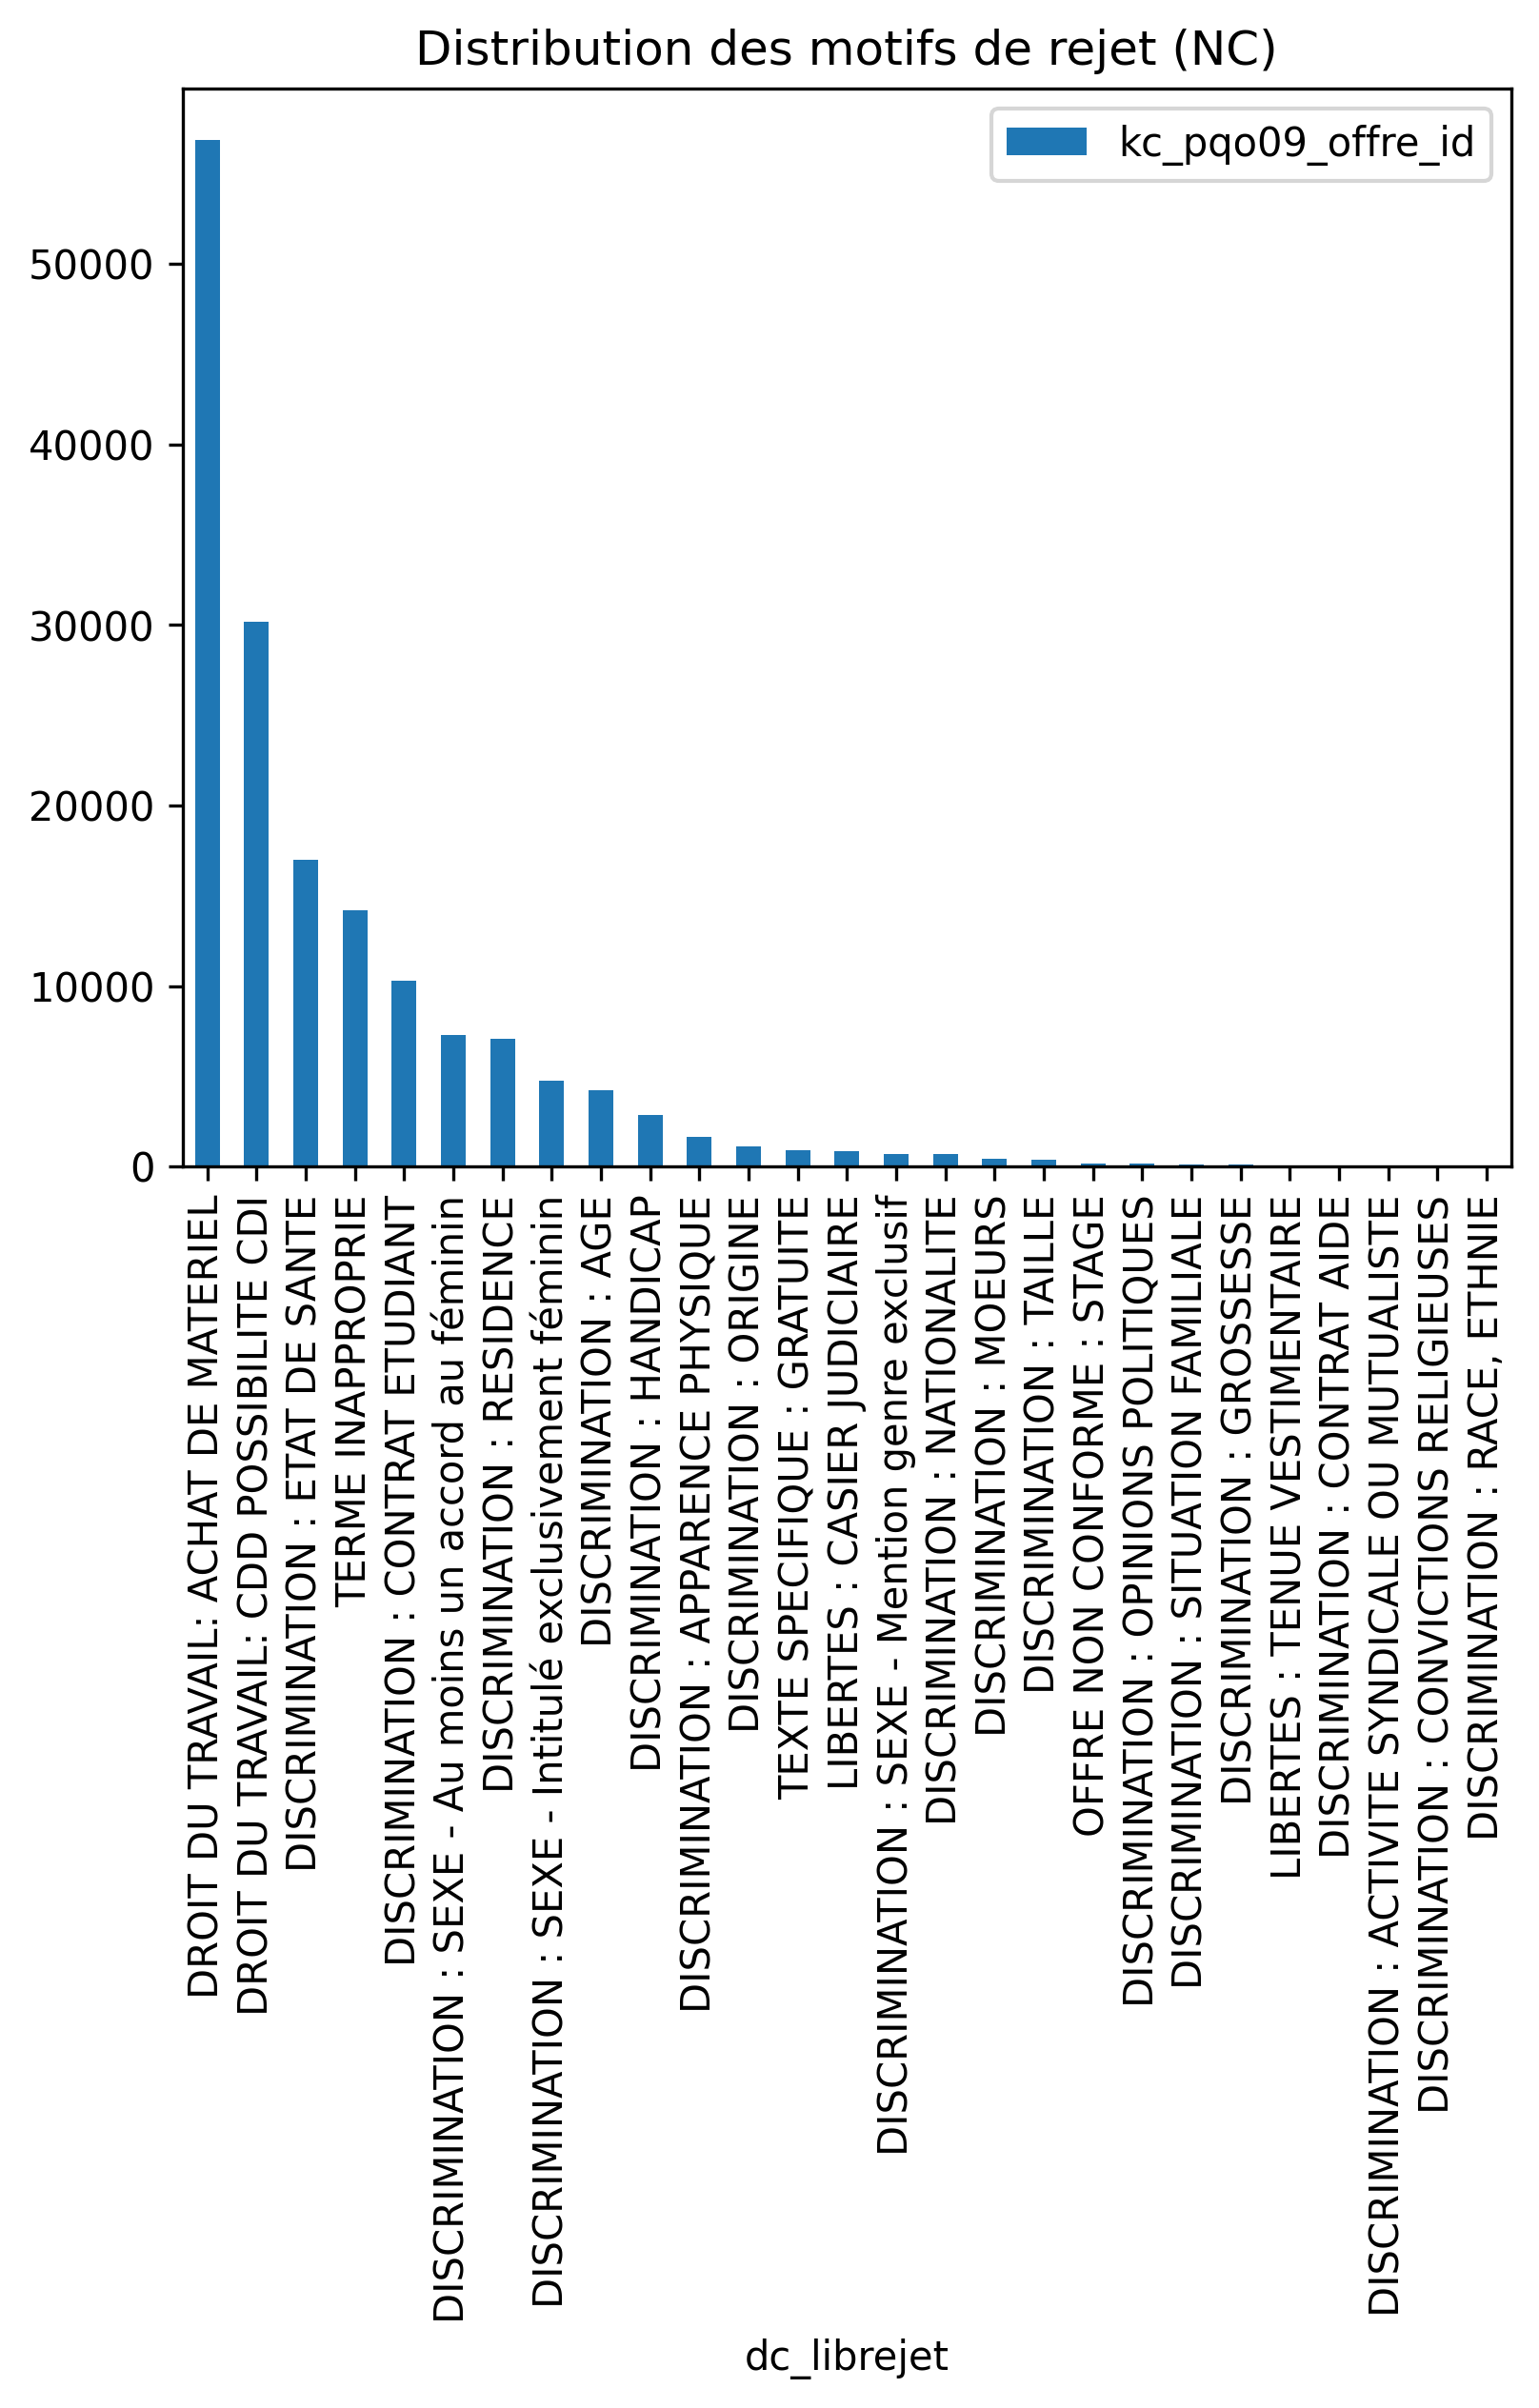
\includegraphics[width=0.8\textwidth]{./S2-Explicabilite_locale/figures/distrib_classes_NC_lego.png}
    \caption{Répartition des motifs de rejet dans les données d'apprentissage. Seules les phrases en alerte (non conformes, NC) sont prises en compte. }
    \label{fig:distrib_nc}
\end{figure}

Le jeu de données de test est constitué de données vérifiées manuellement, et les erreurs du système historiques y sont corrigées. De même, pour les phrases non conformes, les explications associées au motif de rejet sont indiquées sous forme d'ensemble de mots, à l'instar d'un surlignage. Ce travail manuel rend la création de ce jeu de données coûteux, il est donc restreint et composé de $208$ phrases uniquement.

Deux sous-échantillons de cet ensemble de test de 208 phrases sont utilisés. Le jeu de test des bonnes prédictions (BP) est composé de 147 phrases du jeu de test, correctement prédites. Ce jeu de données permet de mesurer la performance des explications lorsque le modèle ne fait aucune erreur. Cela évite que la performance des explications soit affectée dans le cas d'un modèle peu performant. L'ensemble de test de phrases avec différentes explications (DE) est composé de 106 phrases de l'ensemble de test, avec des explications non-identiques entre elles. Ce jeu de données se concentre sur la tâche des utilisateurs qui comparent les explications et évite la situation où les utilisateurs doivent choisir entre des explications uniquement identiques. Ces deux jeux de données se recoupent tel qu'illustré en figure~\ref{fig:lego_test_sets}.

\begin{figure}[htpb!]
    \centering
    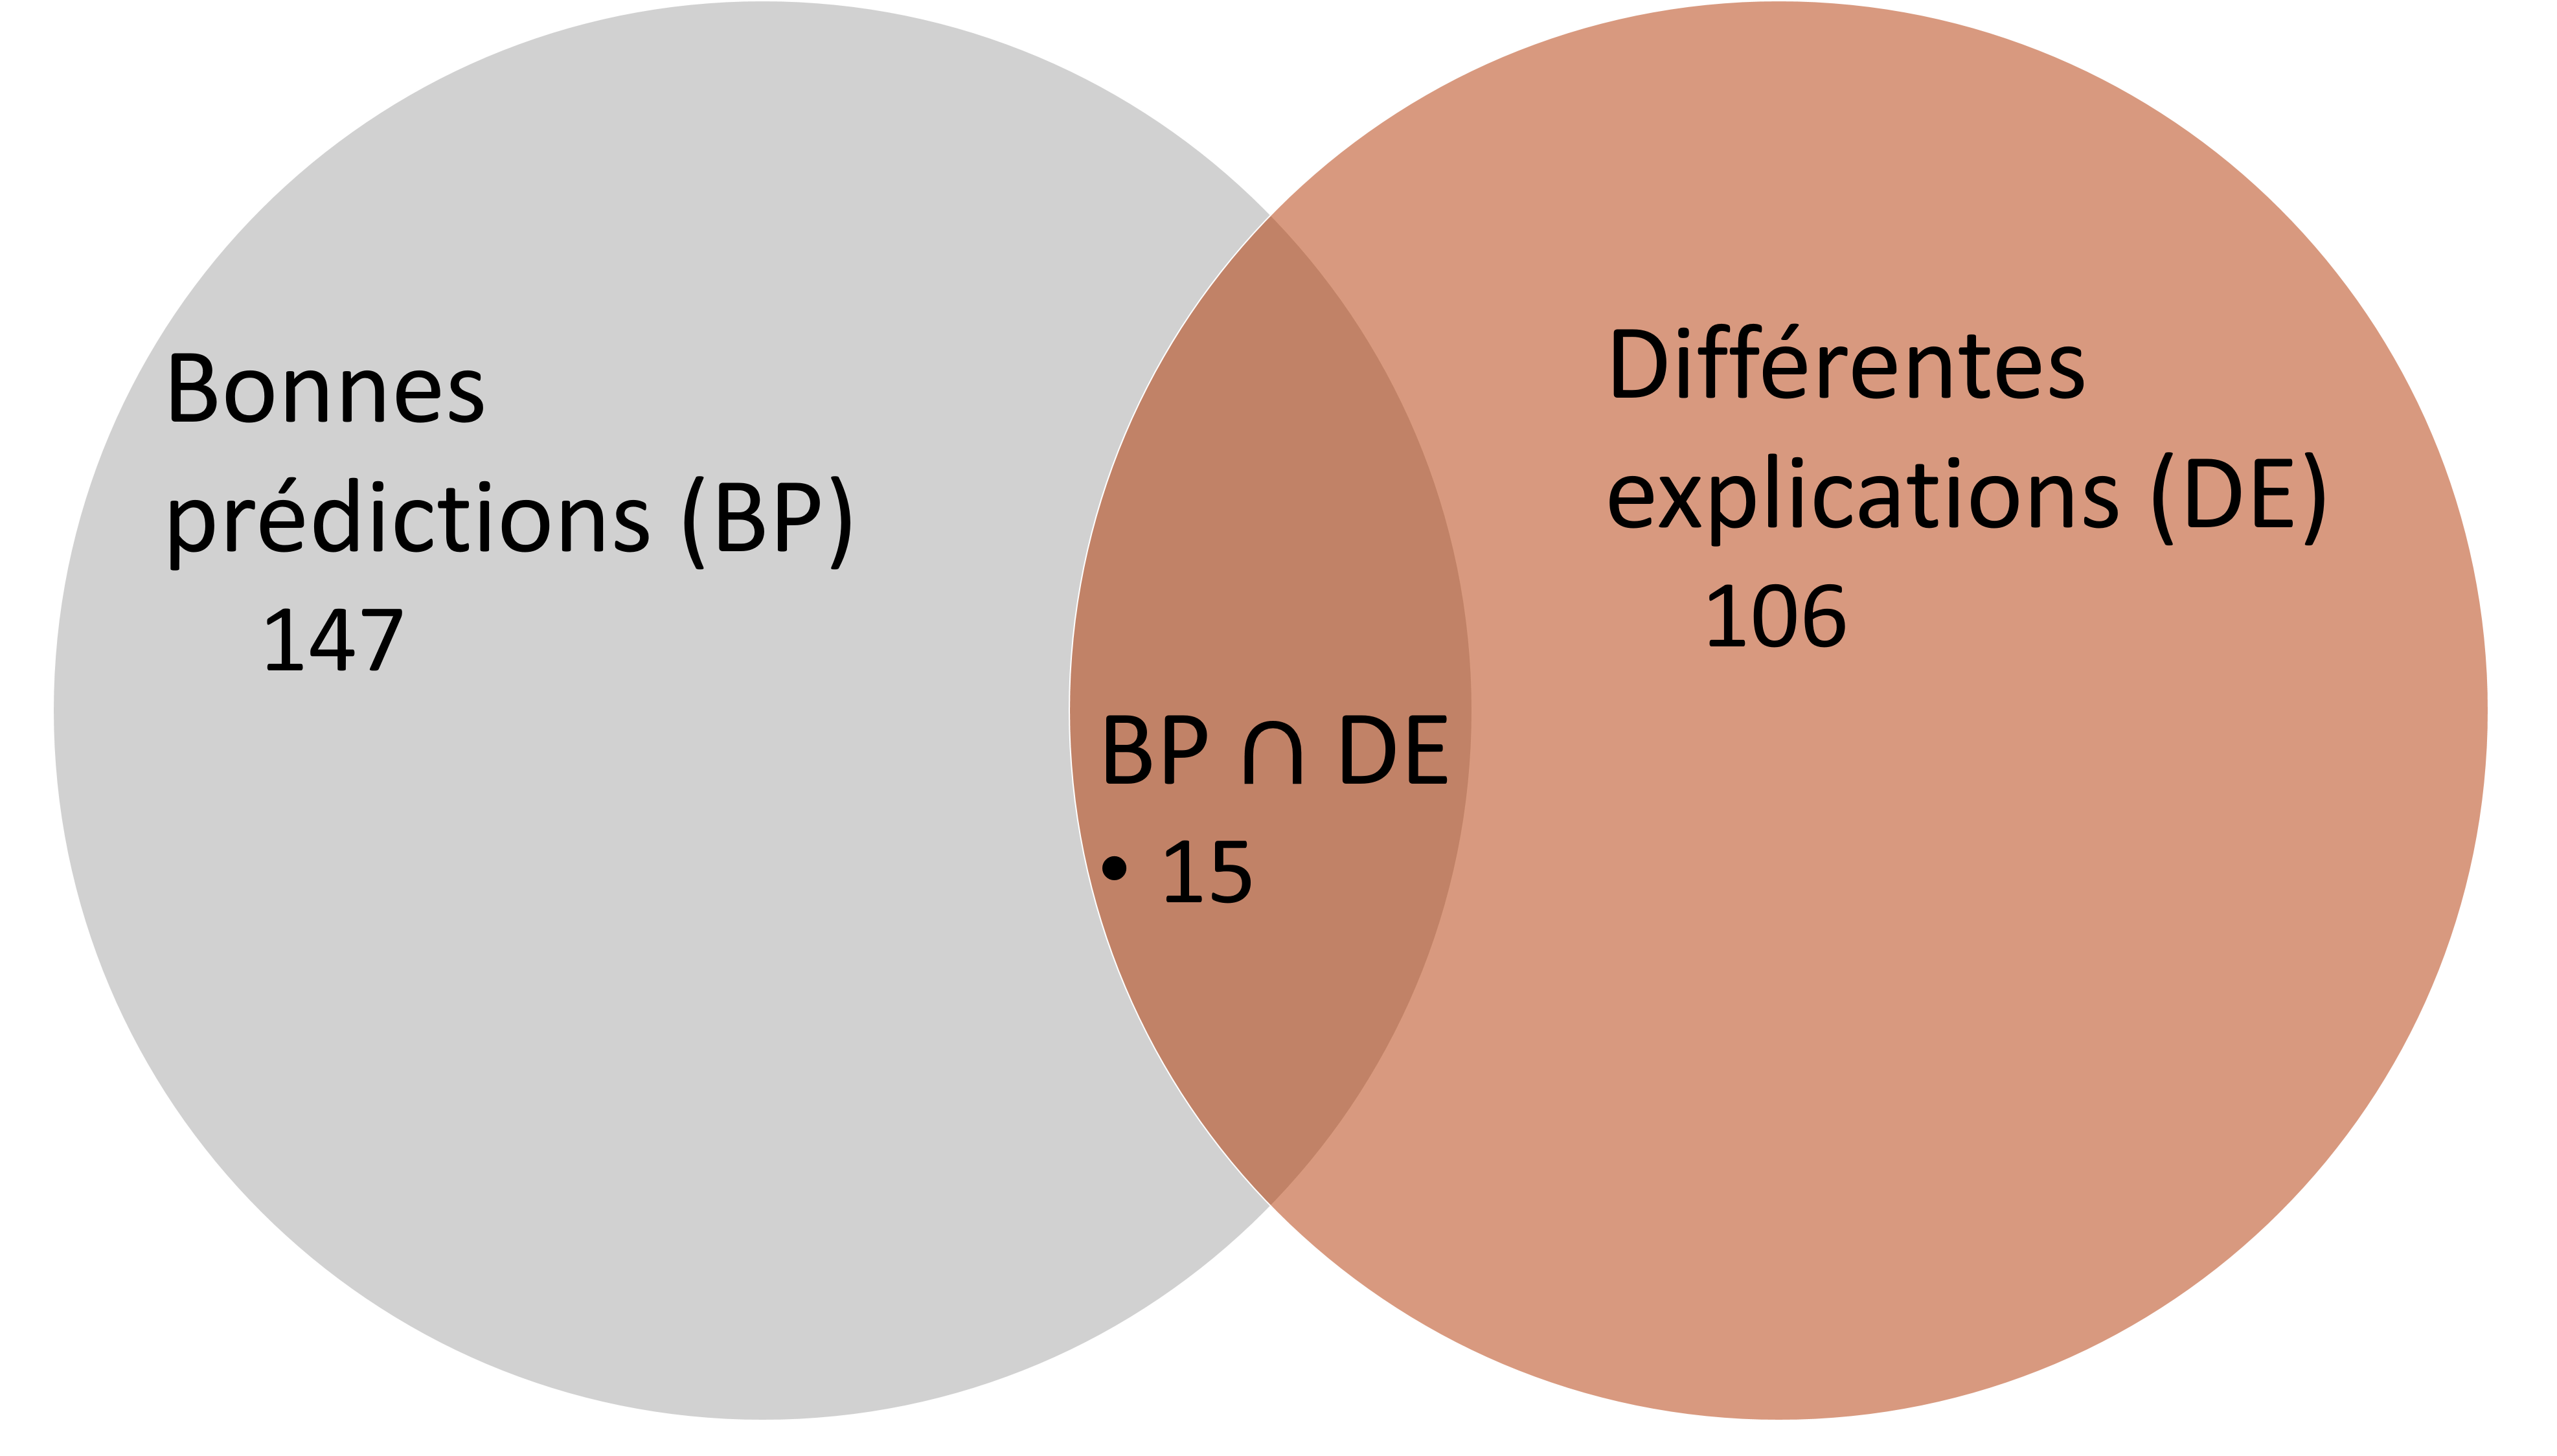
\includegraphics[width=0.6\textwidth]{./S2-Explicabilite_locale/figures/lego_test_sets.png}
    \caption{Ensemble de test de 208 phrases labellisées manuellement. Deux sous ensemble de données en sont extraits : le jeu de test de bonnes prédictions (BP) et composés de différentes explications (ED)}
    \label{fig:lego_test_sets}
\end{figure}

La création de ce jeu de test a soulevé des questionnements, tels que la difficulté de déterminer une explication idéale.

\subsection{Comment collecter les explications de référence} \label{C2:ground_truth}
Générer une explication de référence ou explication attendue peut être fait en s'appuyant sur l'attention humaine~\cite{Mohseni2021}. Il est alors nécessaire de faire appel à des experts du domaine ou, à défaut, à une documentation de référence.
On peut souhaiter obtenir une explication qui réponde à la question ``qu'est-ce qui a été utilisé par le modèle pour donner sa réponse ?''.
Pour obtenir cette explication attendue, une première technique consiste à la demander aux utilisateurs, experts du domaine ou experts du modèle.
Une seconde technique consiste à demander aux experts du domaine de vérifier les résultats des modèles et de voir où se concentre leur attention par oculométrie ou en rendant floues des parties d'une image~\cite{Das2017}. Ces méthodes sont bien adaptées aux explications basées sur les variables d'entrées. Pour des systèmes à base de règles et d'exemples, il est possible, dans un esprit similaire, de demander de rédiger l'explication, ou de la choisir parmi un ensemble pré déterminé.
% definitions
Notre objectif est de comparer les explications générées par un outil à des explications de référence. Pour une instance particulière, nous pouvons séparer les explications humaines en ``explication idéale'' et ``explication attendue''. La différence entre ces termes est définie dans les deux paragraphes suivants.

\paragraph{Une explication idéale} est une explication associée à une donnée d'entrée et sa classification correcte. Elle est idéale parce qu'elle s'applique lorsque la prédiction est juste. Cette explication est basée sur l'expertise du domaine. Si nous voulions entraîner un modèle à donner ces explications, nous les fournirions dans un jeu de données d'entraînement. Elles sont identiques, quel que soit le classifieur utilisé. Dans le cas d'une mauvaise classification, l'explication idéale ne reflète pas le comportement du modèle.

\paragraph{Une explication attendue} est une explication associée à une donnée d'entrée et une classification, que celle-ci soit correcte ou non. L'utilisateur recevant le résultat peut alors espérer obtenir une explication qui soit fidèle au raisonnement, même si erroné, du modèle.

\paragraph{Explications de référence} Nous collectons des explications de référence afin de mesurer des performances de méthode de génération d'explications, peu importe le résultat donné par le classifieur. Dans le chapitre suivant, les explications idéales sont utilisées comme référence dans les expériences réalisées.
Les experts du domaine ayant de fortes contraintes de disponibilité, nous n'avons pas de personnes expertes à disposition pour associer des phrases avec leurs explications.

\paragraph{Documentation métier} Afin de limiter les biais, nous déterminons les explications de référence grâce à la documentation métier. Cette documentation est constituée de documents techniques internes et du Guide d'Aide à la Rédaction des Offres (GARO). Le GARO est un document important pour les conseillers Pôle emploi, mais est peu pratique à utiliser lors des actes métier du fait de sa longueur : 128 pages. Ces documents nous permettent, à titre d'exemple, de déterminer que la discrimination sur le genre des candidats est détectée via l'intitulé de poste d'une offre. Cet intitulé sera alors considéré comme l'explication de référence en cas de rejet. Ces indications permettent de limiter les incertitudes dans la labellisation.

\paragraph{Spécificité du texte} Des questionnements ont émergé lors de cette phase de labellisation manuelle. Les mots porteurs de sens devaient-ils être labellisés ? Quelle est la différence entre ``Une assistante sociale'' et ``assistante sociale'' ? À des fins de simplification, nous avons fait le choix d'ignorer ces mots non porteurs de sens.

\vspace{1cm}
Nous avons défini un cas d'usage et ses données associées. Nous pouvons désormais entraîner un modèle à résoudre notre problème de classification, et générer des explications pour ce modèle.


\section{Génération d'explications par variables d'importance}\label{C2:explications}

Dans cette section, nous appliquons deux méthodes d'explication: la génération d'ancres sur n'importe quel modèle de~\cite{Ribeiro2018} et l'utilisation de l'attention avec un modèle transparent de~\cite{Lin2017}.
% pourquoi
Ce modèle fournit directement des explications locales basées sur les variables d'entrées.

Pour rappel, notre choix a été guidé par les caractéristiques suivantes:
\begin{itemize}
    \item nous ciblons les utilisateurs experts du domaine,
    \item l'explication est reçue lors de la rédaction d'une offre d'emploi,
    \item le modèle de classification est libre de toute contrainte de conception.
\end{itemize}

Nous optons pour des explications de portée locale, donnant des explications au cas par cas. La stratégie est libre, nous choisissons les deux extrêmes : modèle transparent et boîte noire. Nous appliquons deux méthodes d'explication basées sur les variables d'entrée.

Le modèle de référence sera un modèle transparent basé sur l'attention. Son avantage est de permettre la génération d'explications tout en conservant une architecture de réseau de neurone plutôt légère.
La seconde méthode choisie est une méthode boîte noire, la méthode des ancres~\cite{Ribeiro2018}. Ces travaux font suite à LIME~\cite{Ribeiro2016}, une méthode servant de référence en génération d'explications par approche boîte noire.

Les ancres seront générées sur les prédictions du modèle transparent. Ainsi, les deux explications seront basées sur le même modèle, limitant les différences entre explications aux seuls systèmes explicatifs.

En s'inspirant de~\cite{Ribeiro2018} pour l'exemple, prenons la phrase ``Ce film n'est pas mauvais'', qui est classée ``positive'' par un modèle de classification binaire de sentiments, basé sur l'attention. L'explication des ancres serait $ A = \{pas, mauvais \} \rightarrow Positive $. Chaque mot de la phrase posséderait un poids d'attention, et ``pas'' et ``mauvais'' auraient les poids les plus élevés. Les deux méthodes extraient des ensembles de mots d'intérêt. % TODO ajout formalisation sous forme d'équation

% plan
Dans un premier temps nous présenterons le modèle transparent à attention, puis nous présenterons les ancres qui permettront d'expliquer ce même modèle.

\subsection{Attention} \label{C2:attention}

% Quoi
Le mécanisme d'attention consiste à apprendre une couche spécifique d'attention à un modèle. Il est ainsi possible d'extraire des poids d'attentions associés aux variables d'entrée d'une instance, qui correspondent à une pondération de focalisation du modèle.

% comment
Suivant les recherches de~\cite{Lin2017}, nous concevons un réseau de neurones avec une architecture spécifique. Celle-ci combine un bi-LSTM, couche adaptée aux traitement de textes, et le mécanisme d'attention~\cite{Lin2017}. Les détails de l'architecture sont présentés dans le tableau ci-dessous (cf. Table~\ref{tab:model_architecture}).

\begin{table}[htb!p]
\caption{Architecture du réseau de classification à attention pour le cas d'usage LEGO.}\label{tab:model_architecture}
\begin{tabular}{|l|p{0.23\textwidth}|p{0.18\textwidth}|p{0.45\textwidth}|}
\hline
\textbf{ID} & \textbf{Type de couche} & \textbf{Paramètres} & \textbf{Commentaires} \\ \hline
1 & Couche d'entrée    & 80               & La taille est le nombre de mots dans les textes \\ \hline
2 & Plongement de mots & 300              & Plongement de mots GloVe\\ \hline
3 & Bi-LSTM            & $u=$50           & La sortie est la matrice d'états cachés H \\ \hline
4 & Couche dense 0     & $d_a=$300        & Activation $tanh$ \\ \hline
5 & Couche dense 1     & $r=$1            & La sortie est la matrice d'attention A\\ \hline
6 & Représentation     & sortie: $[2u,r]$ & Combinaison de l'attention et de la couche cachée, $M=A^T*H$ \\ \hline
7 & Sortie             &  28              & Couche de sortie \\ \hline
\end{tabular}
\end{table}

Le réseau a été adapté au cas d'usage, les dimensions des couches et autres commentaires sur l'architecture sont détaillés dans le tableau~\ref{model_architecture}. Dans ce tableau, $u$ est la taille du bi-LSTM, $d_a$ la taille de la couche dense 0, r le nombre de têtes d'attention et M la matrice de représentation. Le mécanisme d'attention aboutit à une matrice d'attention A, qui est la sortie de la couche 5 (cf. Table~\ref{model_architecture}).
L'optimisation des hyper paramètres $u$, $d_a$ a été effectuée en premier, puis le taux d'apprentissage a été ajusté sur l'intervalle $[5.10^{-5},10^{-1}]$.
Les mots d'intérêt sont filtrés en utilisant un seuil $t$ sur les valeurs d'attention. Lorsque le modèle ne prédit aucun rejet, l'explication est vide.

Pour ce classifieur, la matrice de plongement de mots utilisée est un plongement GloVe (``Global Vectors for Word Representation'') de 300 dimensions\footnote{\url{https://dl.fbaipublicfiles.com/fasttext/vectors-crawl/cc.fr.300.vec.gz}}. Le taux d'apprentissage de $0,0005$ est déterminé par essais successifs. Ce réseau atteint un taux de reconnaissance de $83,67\%$ sur son ensemble de test.

Un seuil $t$ est utilisé afin de filtrer les mots. $t$ est déterminé en optimisant l'IOU sur un ensemble de test de 208 phrases, en comparant les explications à attention et la référence. Les résultats sont présentés dans le graphique de la Figure~\ref{fig:threshold}. Ils indiquent que les mots dont l'attention est supérieure ou égale à $0,15$ constituent une bonne explication. Nous générons ainsi des explications avec les seuils de valeurs $t = 0,15$.

\begin{figure}[t]
     \setlength{\belowcaptionskip}{-20pt}
   \begin{center}
     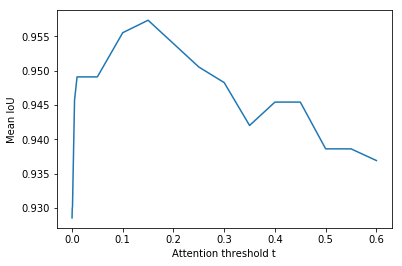
\includegraphics[height=4.5cm]{./S2-Explicabilite_locale/figures/plot_iou_threshold.png}
     \caption{Similarité (IOU) moyenne entre les explications générées et de référence dans l'ensemble de test, pour un seuil d'attention $t$ variable. Les mots dont l'attention est supérieure ou égale à $t$ forment l'explication. Le premier point est à $10^-4$. }\label{fig:threshold}
   \end{center}
\end{figure}

\paragraph{Avantages et inconvénients}
% avantages
Cette méthode de détection des mots importants a pour avantage de s'appuyer directement sur le fonctionnement interne du réseau. Le mécanisme d'attention permet de pondérer les entrées selon leur importance, avec pour objectif l'amélioration des performances du réseau. Ces pondérations sont ajustées lors de la phase d'entraînement du modèle, en optimisant les résultats de la tâche de classification. Ainsi, la génération d'explications ne nécessite pas de données supplémentaires. En faisant de l'anthropomorphisme, le réseau ``apprend de lui-même à focaliser son attention sur certains éléments''.
Le second avantage de cette méthode est qu'elle ne nécessite pas de calcul après entraînement, hormis celui de l'inférence. Plus exactement, dans l'implémentation effectuée, le modèle est appelé une fois pour obtenir le résultat, et si la phrase est rejetée, une seconde fois pour extraire les poids d'attention.

% inconvénients
Cette méthode souffre toutefois des critiques énoncées dans le Chapitre~\ref{C1}, en section~\ref{C1:debat}. Elle n'est pas toujours fiable, l'attention apprise différant parfois fortement des autres méthodes d'explicabilité, qui ont acquis leur réputation dans la communauté scientifique. Si cette méthode limite les calculs lors de l'inférence, elle nécessite tout de même d'alourdir le modèle avec les couches 4, 5 et 6 du tableau~\ref{tab:model_architecture} .


\subsection{Ancres}

% Quoi
Les ancres sont des règles extraites par analyse d'un ensemble de données générées et leurs sorties associées. Les données sont générées par perturbation de l'instance à expliquer. Les masquages permettent de déterminer quelles instances ont un impact sur le résultat final du modèle.
% comment
Nous générons les ancres avec la bibliothèque python\footnote{\url{https://github.com/marcotcr/anchor}} développée par les auteurs de~\cite{Ribeiro2018}. Afin de réduire les écarts d'explications aux seules performances des méthodes de génération des explications, les ancres sont générées en utilisant le modèle à attention développé en section~\ref{C2:attention}. Les paramètres de génération des ancres sont détaillés dans la tableau ci-dessous~\ref{tab:ancres_params}.

\begin{table}[htb!p]
\caption{Paramètre de génération des ancres pour le cas d'usage LEGO.}\label{tab:ancres_params}
\begin{tabular}{|p{0.15\textwidth}|p{0.10\textwidth}|p{0.55\textwidth}|}
\hline
\textbf{Paramètre} & \textbf{Valeur} & \textbf{Commentaires} \\ \hline
Seuil              & $0,95$ & Précision minimale requise pour ajouter un nouveau mot \\ \hline
Delta              & $0,1$  & Marge d'erreur  \\ \hline
Tau                & $0,15$ & Critère de précision de l'ancre\\ \hline
Taille de faisceau & $4$ & Taille du faisceau de recherche, sélectionne $N$ candidats à chaque tour\\ \hline
Taille de lot      & $100$  & Nombre de données générées  \\ \hline % (def. 10)
\end{tabular}
\end{table}

Dans un premier temps, rappelons quelques notations. Un domaine d'application est l'ensemble des instances pour lesquelles une règle A est vérifiée, $A(.)=1$. A est une ancre si l'ensemble $\mathbb{E}_{D(Z|A)}$ des instances du domaine d'application sont classés comme l'instance à expliquer $x$, avec un taux supérieur à la précision souhaitée $\tau$. On peut le formaliser par l'équation suivante :
\begin{equation}
     \mathbb{E}_{D(Z|A)} [ \mathbbm{1}  _{f(x)=f(z)}] \geq \tau
\end{equation}
Calculer la précision d'une ancre n'est pas possible pour un modèle $f$ et un ensemble $D$ donnés.
Nous calculons alors la probabilité que l'ancre corresponde au critère de précision $\tau$ en acceptant une marge d'erreur $\delta$.
\begin{equation}
    P(prec(A) > \tau) \geq 1 - \delta
\end{equation}

On cherche enfin à conserver les ancres qui couvrent un plus grand nombre possible d'instances. La recherche s'effectue en partant d'une ancre vide, et en créant $N$ ancres candidates par l'ajout de variables.
Les paramètres du tableau~\ref{tab:ancres_params} sont identiques aux paramètres de base des ancres. Toutefois nous avons dû augmenter la taille du faisceau de recherche, afin d'améliorer les performances.

\paragraph{Avantages et inconvénients}
% avantages
La méthode des ancres permet de générer des explications sans s'inquiéter du fonctionnement interne du modèle. Les performances de ce dernier ne sont donc pas altérées. Les explications générées ont un cadre d'application défini.

% inconvénients
Cependant cette méthode nécessite d'appeler le modèle un nombre important de fois. Elle est donc couteuse en calcul à chaque génération d'explication, et fonctionne mal sur un nombre trop important de variables d'entrées; dans notre cas, sur les phrases longues. Enfin, il y a un risque de s'appuyer sur des comportements erratiques du modèle voire de créer des instances adversariales, en définissant le comportement sur un domaine d'application constitué de données hors distribution.

\paragraph{Explications générées}
Ces deux méthodes permettent de générer différentes explications présentées dans le tableau~\ref{explications_lego}. Les explications par les ancres sont basées sur le modèle à attention, et deux explications reposent sur le mécanisme d'attention. Lorsque le modèle ne prédit aucun rejet, les explications générées sont forcées d'être vides.

\begin{table}[h!tpb]
\caption{LEGO : phrases avec leurs différentes explications. Le texte est au-dessus des autres informations. Les phrases portent respectivement les numéros 0 et 73 du jeu de données LEGO - DE.}\label{explications_lego}
\begin{tabular}{|p{0.15\textwidth}|p{0.18\textwidth}|p{0.2\textwidth}|p{0.17\textwidth}|p{0.15\textwidth}|}
  \cline{1-5}
  \textbf{Rejet} & \textbf{Référence} & \textbf{Ancres} & \textbf{Attention 0.15} & \textbf{Attention 0.5} \\ \hline
  \multicolumn{5}{|p{0.95\textwidth}|}{``[...] Notre agence de Saint-Medard-en-Jalles recherche une Assistante Administrative pour completer son equipe.''}\\ \hline
  Genre& ['assistante administrative'] & ['recherche', 'Assistante', 'Jalles'] & ['assistante', 'administrative'] & ['assistante'] \\ \cline{1-5}
  \multicolumn{5}{|p{0.95\textwidth}|}{``Poste en CDD renouvelable en cdi.''}\\ \hline
  CDD possibilit\'e CDI\footnotemark[3] & ['CDD renouvelable en cdi'] & ['CDD renouvelable', 'cdi'] & ['cdi'] & ['cdi'] \\ \cline{1-5}
\end{tabular}
\end{table}

\footnotetext[3]{Contrat à durée déterminée conduisant à un contrat à durée indéterminée}

Nous avons détaillé les méthodes de génération d'explication permettant de détecter les mots importants dans les phrases d'offres d'emploi. Dans la section suivante, nous présentons différentes interfaces d'explications pour le cas d'usage LEGO.


\section{Visualisations pour les explications locales} \label{C2:demonstrateur}

Les explications étant à destination d'humains, nous détaillons dans cette section la création d'un démonstrateur et des pistes de visualisations à présenter aux utilisateurs experts du domaine. L'objectif est de conduire un test d'utilisabilité à partir de ces visualisations pour déterminer quelles interfaces nous allons développer. Ces interfaces permettront la collecte des préférences utilisateurs.

% Quoi
Le démonstrateur est un prototype d'interface, reprenant des éléments de l'interface d'origine présentée en figure~\ref{fig:ihm_DUNE}. Dans un premier temps, nous reprenons l'interface la plus simple possible, cf. figure~\ref{fig:demo_no_exp}. Le premier élément repris est le champ de texte pour le descriptif du poste. Nous ajoutons un bouton pour lancer la prédiction, remplaçant le bouton ``poursuivre'' de l'interface d'origine.

 \begin{figure}[htpb!]
     \centering
     \begin{subfigure}[b]{0.48\textwidth}
        \centering 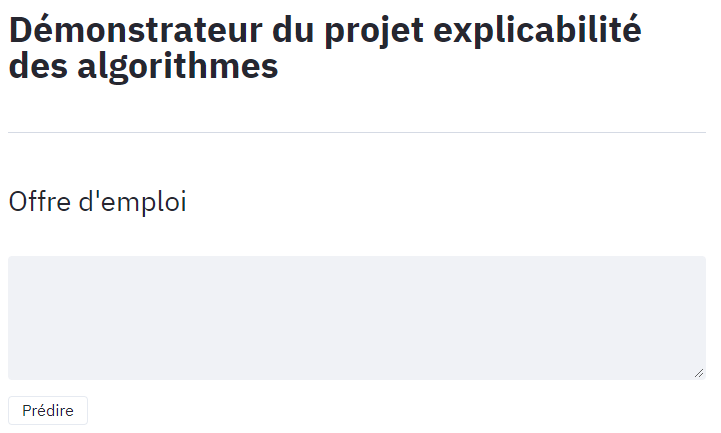
\includegraphics[width=\textwidth]{S2-Explicabilite_locale/figures/demo_empty.png}
        \caption{Démonstrateur avant prédiction}
        \label{fig:demo_empty}
     \end{subfigure}
     ~
     \begin{subfigure}[b]{0.48\textwidth}
        \centering 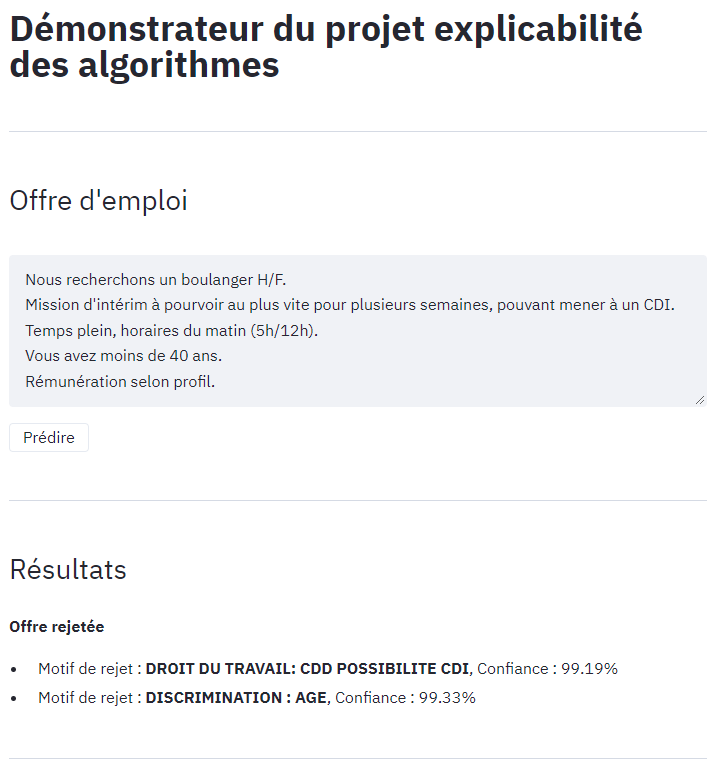
\includegraphics[width=\textwidth]{S2-Explicabilite_locale/figures/demo_base.png}
        \caption{Démonstrateur après prédiction, sans explications}
        \label{fig:demo_base}
     \end{subfigure}
     ~
     \caption{Démonstrateur présentant l'interface homme-machine du système d’explications locales, sans explications.
     }\label{fig:demo_no_exp}
 \end{figure}

% Comment
Lorsque l'utilisateur clique sur le bouton ``Prédire'', le résultat du modèle d'IA apparaît dans un encart sous le texte, présenté dans la figure~\ref{fig:demo_base}. Cette organisation diffère légèrement du bandeau explicatif situé au-dessus du texte dans l'interface d'origine en figure~\ref{fig:ihm_DUNE}, mais permet une lecture de haut en bas.
Le bandeau de résultat comprend un score de confiance du modèle. Plus le pourcentage est proche de 100\%, plus la décision est tranchée. Un score plutôt faible, vers 50\%, constitue une alerte.
Les développements se basent sur les retours du test d'utilisabilité présenté dans le chapitre suivant, en section~\ref{C3:test_u}.
Ils permettent la présentation aux utilisateurs des explications générées en section précédente, afin de collecter leurs préférences.
Nous ajoutons ensuite à ce démonstrateur différents types d'explications locales aux utilisateurs, afin de leur permettre d'interagir en se rapprochant légèrement des conditions d'usage réel, tout en restant simple à développer et maintenir. Les visualisations proposées sont une explication par surlignage de la phrase puis des mots déclenchant le rejet, d'une règle métier associée et enfin d'un contre-exemple.% Todo keep ? meh.

 % plan
Les différentes pistes envisagées sont abordées avec leurs avantages et inconvénients.
La première interface présentée est celle mettant en avant les phrases illégales. Puis vient l'explication basée sur les mots importants de cette phrase, suivie de celles basées sur les règles métiers, et les contre-exemples.

\subsection{Préparation des illustrations} \label{C2:preparation}

La préparation des illustrations est la première étape pour réaliser le test d'utilisabilité. Elles sont réalisées eu égard aux préoccupations du public cible; les experts du domaine. Ces objectifs sont les suivants :
\begin{itemize}
    \item corriger une offre rejetée,
    \item détecter si l’outil se trompe,
    \item créer de la confiance en l'outil.
\end{itemize}

Les illustrations prennent en compte différents éléments de l'interface d'origine, présentée dans le chapitre 2. À savoir le bandeau d'alerte, la raison de l'alerte et le champ de descriptif du poste.
Nous reprenons ces éléments et les repositionnons dans les illustrations, en partant sur quatre pistes, à savoir la mise en avant d'une phrase, d'un mot, d'un exemple et d'un contre-exemple. Chaque piste est illustrée et détaillée dans les paragraphes ci-après.

\paragraph{Illustration d'explication par phrase}
% Quoi
La première proposition d'illustration est la mise en avant de la ou les phrases entraînant le rejet d'une offre.
% Pourquoi
Elle permet de donner le contexte du rejet, le texte étant analysé phrase par phrase. L'explication est donc à son niveau de contexte le plus large, laissant au receveur de l'explication le soin de comprendre le détail.
% variantes
Pour mettre en avant une phrase, de nombreuses options sont possibles. Nous en avons prédéterminé trois, présentées dans la figure~\ref{fig:prototype_phrase}.
Il est ainsi possible de la surligner pour indiquer son rejet, comme dans la figure~\ref{fig:prototype_phrase1}.
De même, pour faire apparaître plusieurs éventuels motifs de rejet pour une même phrase, nous pouvons la souligner comme présenté dans la figure~\ref{fig:prototype_phrase2}.
Enfin, une autre proposition est d'afficher une bulle explicative lorsque le curseur de l'utilisateur survole la phrase, idée schématisée dans l'illustration en figure~\ref{fig:prototype_phrase3}.

% illustration
\begin{figure}[htpb!]
    \centering
    \begin{subfigure}[b]{\textwidth}
        \centering 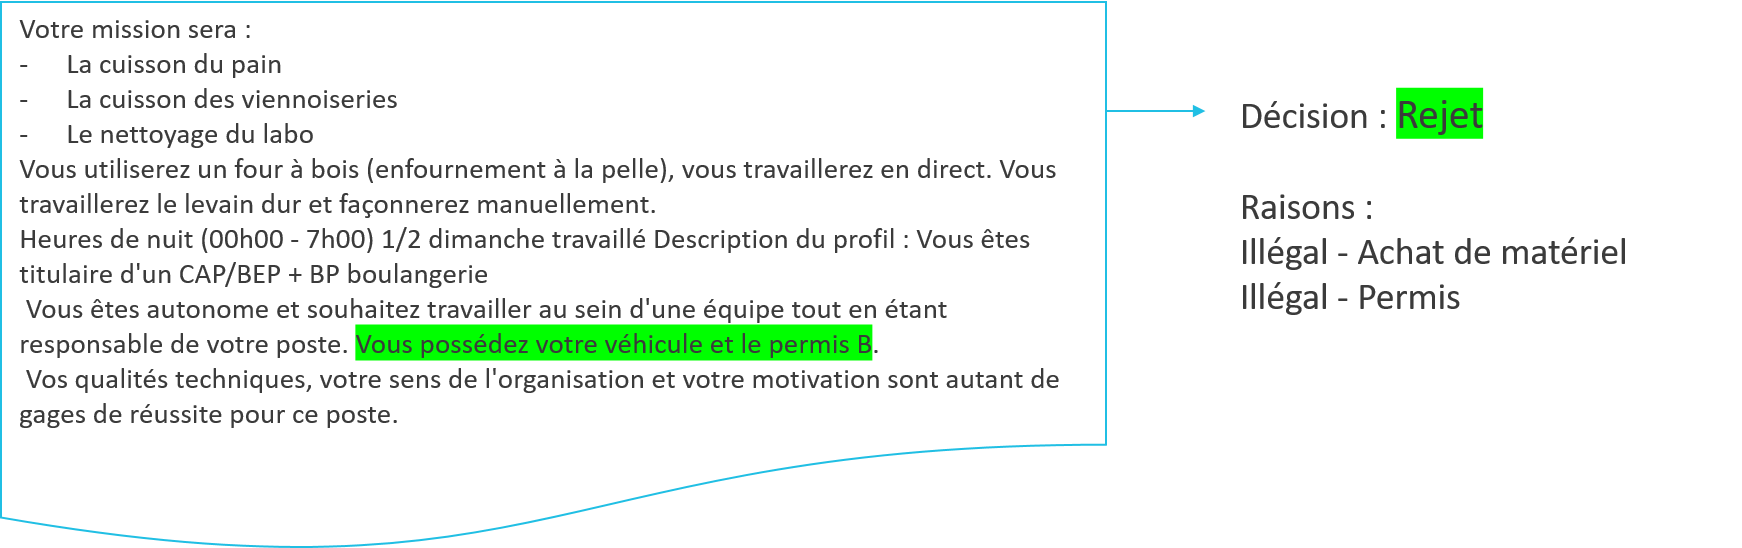
\includegraphics[width=\textwidth]{S2-Explicabilite_locale/figures/prototype_phrase1.png}
        \caption{Mise en avant d'une phrase rejetée par surlignage}
        \label{fig:prototype_phrase1}
    \end{subfigure}
    ~
    \begin{subfigure}[b]{\textwidth}
        \centering 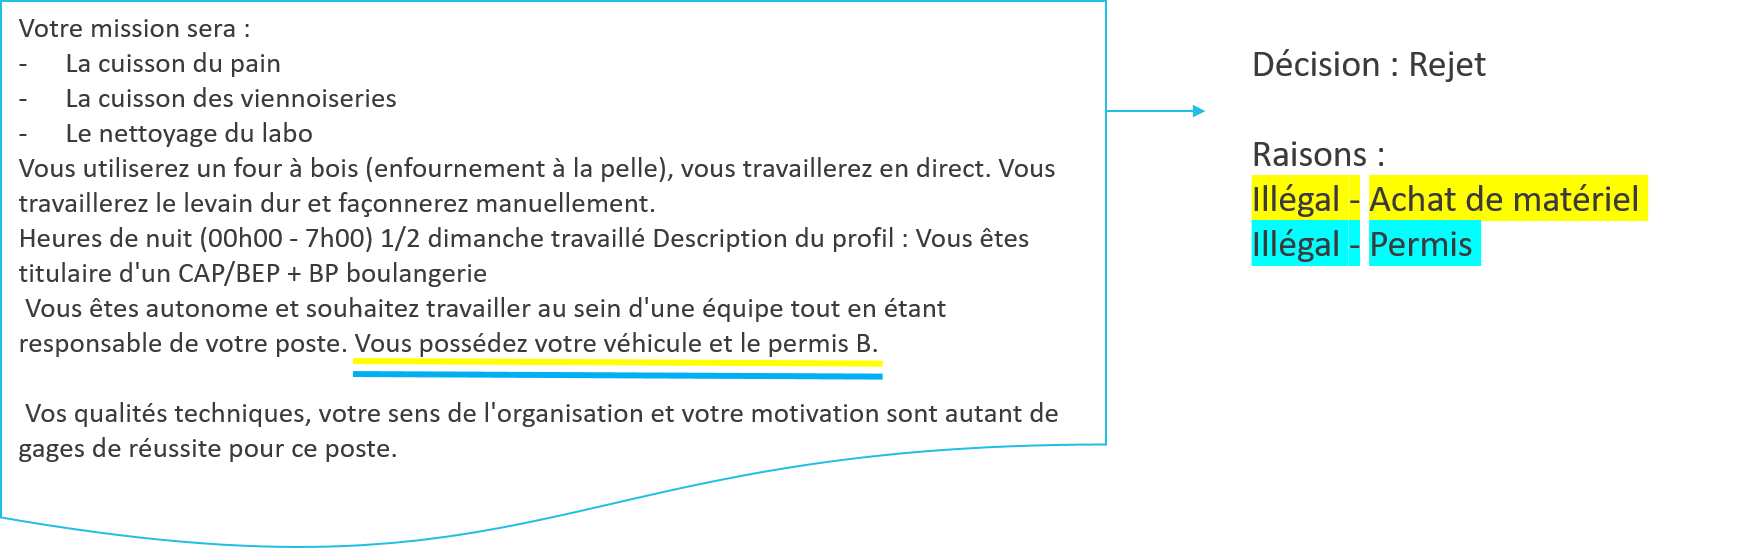
\includegraphics[width=\textwidth]{S2-Explicabilite_locale/figures/prototype_phrase2.png}
        \caption{Mise en avant d'une phrase rejetée par soulignage}
        \label{fig:prototype_phrase2}
    \end{subfigure}
    ~
    \begin{subfigure}[b]{\textwidth}
        \centering 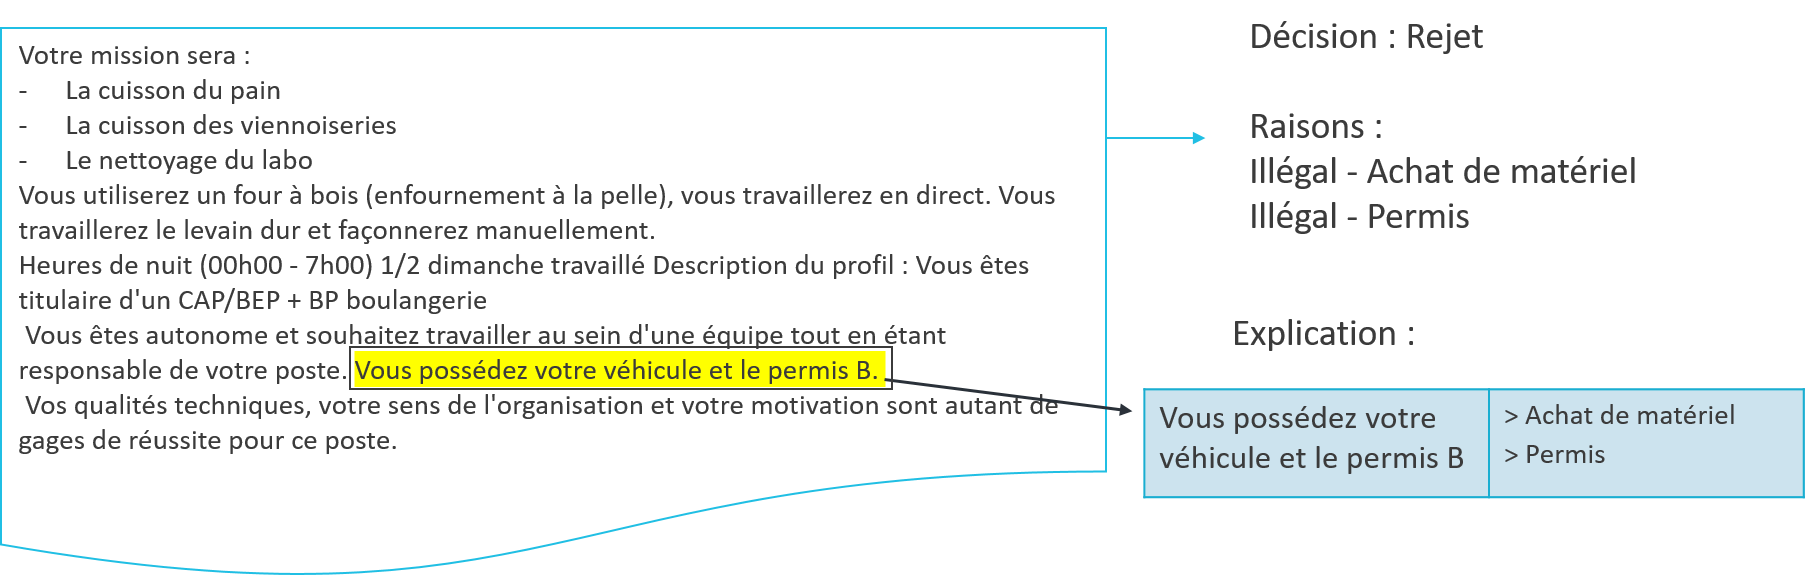
\includegraphics[width=\textwidth]{S2-Explicabilite_locale/figures/prototype_phrase3.png}
        \caption{Mise en avant d'une phrase rejetée via surlignage et bulle d'information apparaissant au survol de la phrase}
        \label{fig:prototype_phrase3}
    \end{subfigure}
    ~
    \caption{Illustrations de variantes d'une explication par la mise en avant d'une phrase.
    }\label{fig:prototype_phrase}
\end{figure}

\paragraph{Illustration d'explication par mot}
 % Quoi
 La seconde proposition consiste à mettre en avant les mots de la phrase responsables du rejet.
 % Pourquoi
 C'est l'explication avec le plus de précision, les phrases étant parfois longues. En contrepartie c'est l'explication qui donne le moins de contexte. Elle est également très proche du système expert d'origine, celui-ci étant basé sur des expressions régulières. Ce système original remontait donc des mots ou ensemble de mots prédéterminés et consignés dans un cahier des charges, sans tenir compte du contexte.
 % variantes
 Similairement aux phrases, nous proposons différentes variantes de maquette. Ces variantes sont illustrées dans la figure~\ref{fig:prototype_mot}. La figure~\ref{fig:prototype_mot1} montre les mots soulignés. Les mots peuvent être surlignés, avec une bulle indiquant le motif de rejet affiché au survol du mot en question, comme illustré en figure~\ref{fig:prototype_mot2}. Enfin, pour se rapprocher de l'interface d'origine, il est également proposé d'afficher le ou les mots en questions en dehors du champ texte, dans un bandeau à part. Cette maquette est illustrée en figure~\ref{fig:prototype_mot3}.
 % illustration
 \begin{figure}[htpb!]
     \centering
     \begin{subfigure}[b]{\textwidth}
        \centering 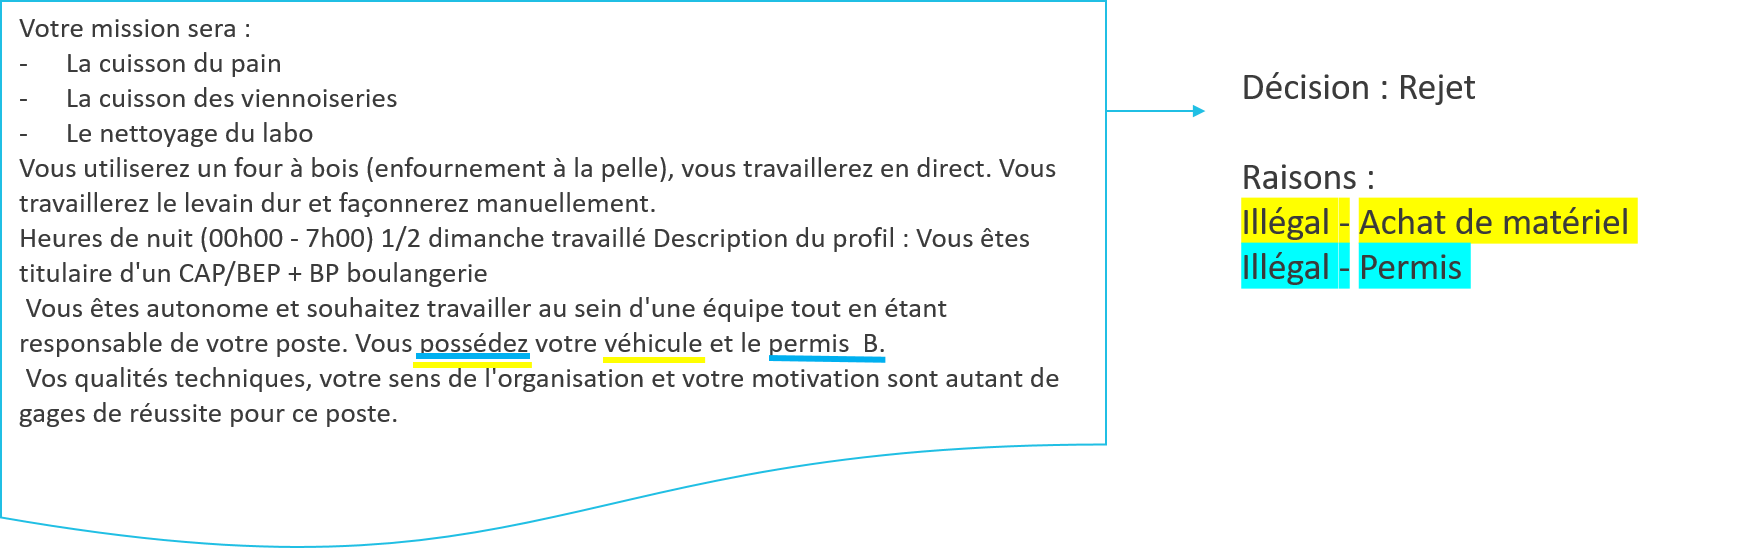
\includegraphics[width=\textwidth]{S2-Explicabilite_locale/figures/prototype_mot1.png}
        \caption{Mise en avant de mots par soulignage}
        \label{fig:prototype_mot1}
     \end{subfigure}
     ~
     \begin{subfigure}[b]{\textwidth}
        \centering 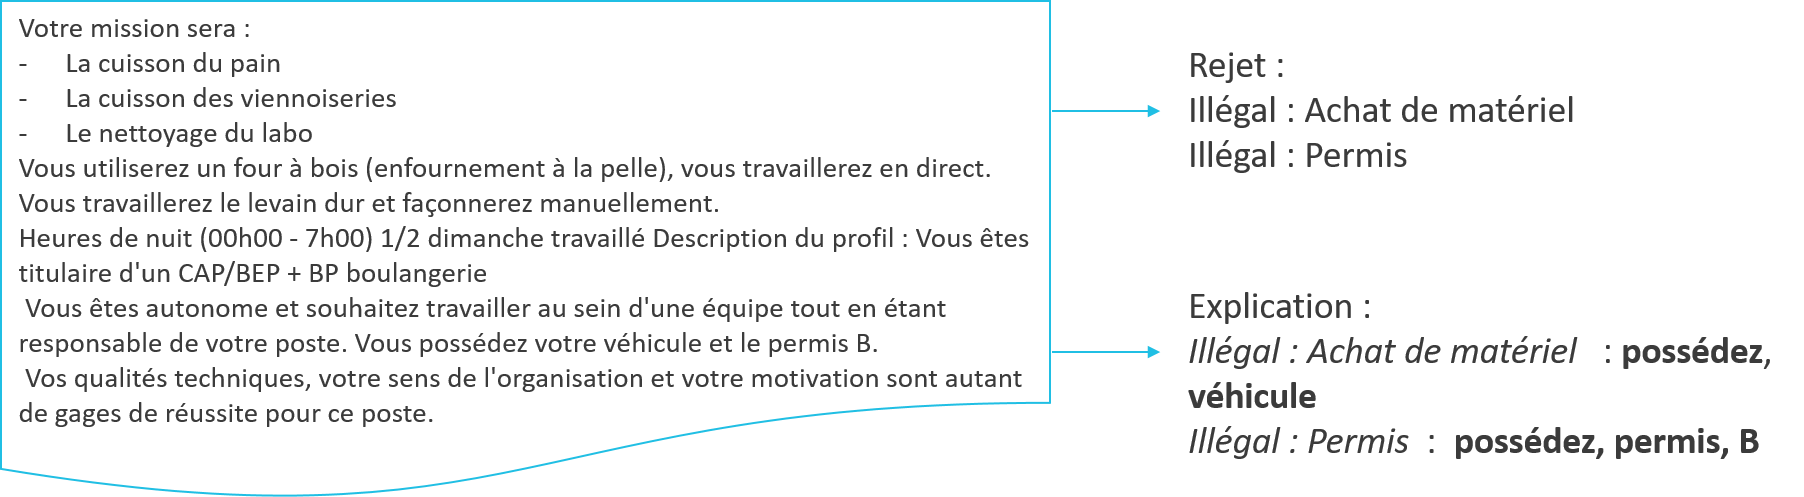
\includegraphics[width=\textwidth]{S2-Explicabilite_locale/figures/prototype_mot3.png}
        \caption{Mise en avant de mots par affichage dans un bandeau externe}
        \label{fig:prototype_mot2}
     \end{subfigure}
     ~
     \begin{subfigure}[b]{\textwidth}
        \centering 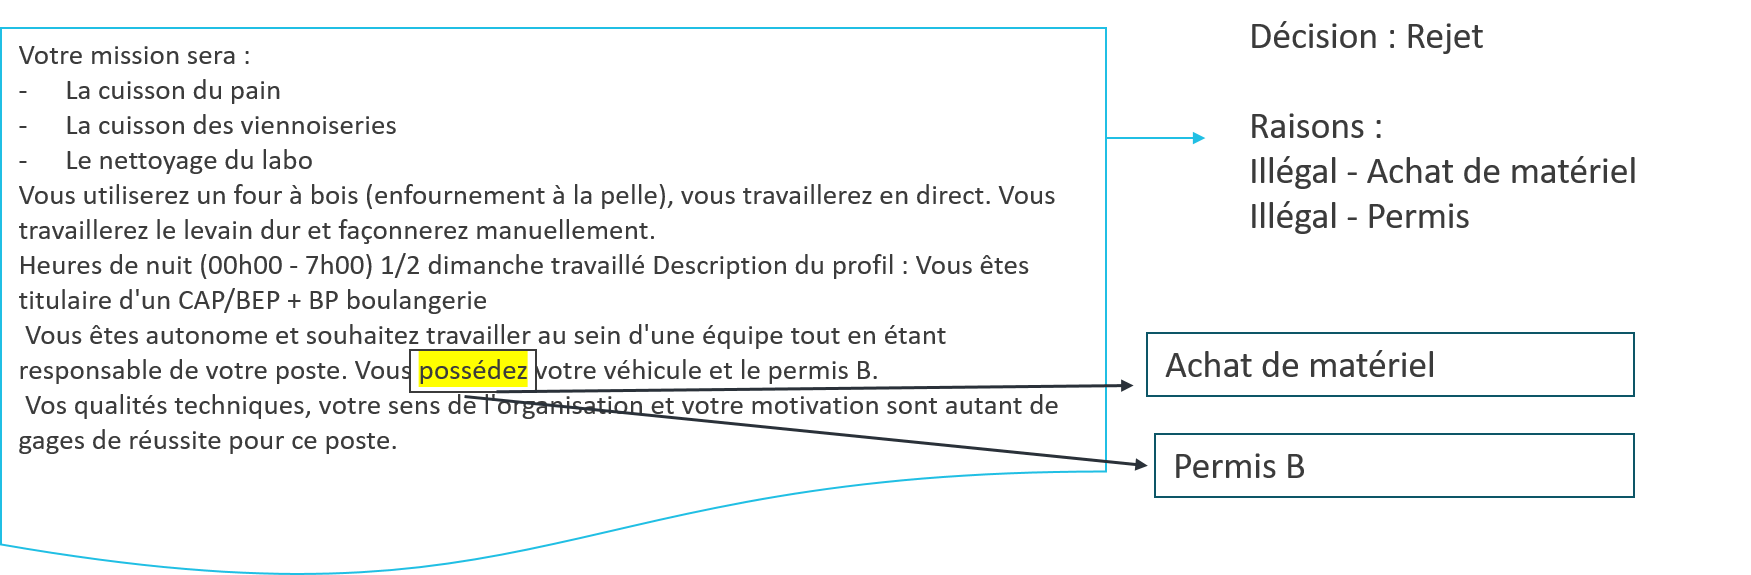
\includegraphics[width=\textwidth]{S2-Explicabilite_locale/figures/prototype_mot2.png}
        \caption{Mise en avant de mots via surlignage et bulle d'information apparaissant au survol des mots}
        \label{fig:prototype_mot3}
     \end{subfigure}
     ~
     \caption{Illustrations de variantes d'une explication par la mise en avant de mots.
     }\label{fig:prototype_mot}
 \end{figure}

\paragraph{Illustration d'un exemple}
 % Quoi
 La troisième maquette proposée est l'explication par l'exemple, affichant pour chaque phrase rejetée une phrase proche, elle aussi classée sur le même motif de rejet.
 % Pourquoi
 Ce type d'explication permet à l'utilisateur d'avoir un exemple de phrase qui entraîne un rejet, et qui comportera sans doute des mots identiques ou similaires à la phrase responsables du rejet. La figure~\ref{fig:prototype_exemple} présente l'illustration proposée, avec une phrase proposée pour chaque motif de rejet détecté.
 % illustration
 \begin{figure}[htpb!]
     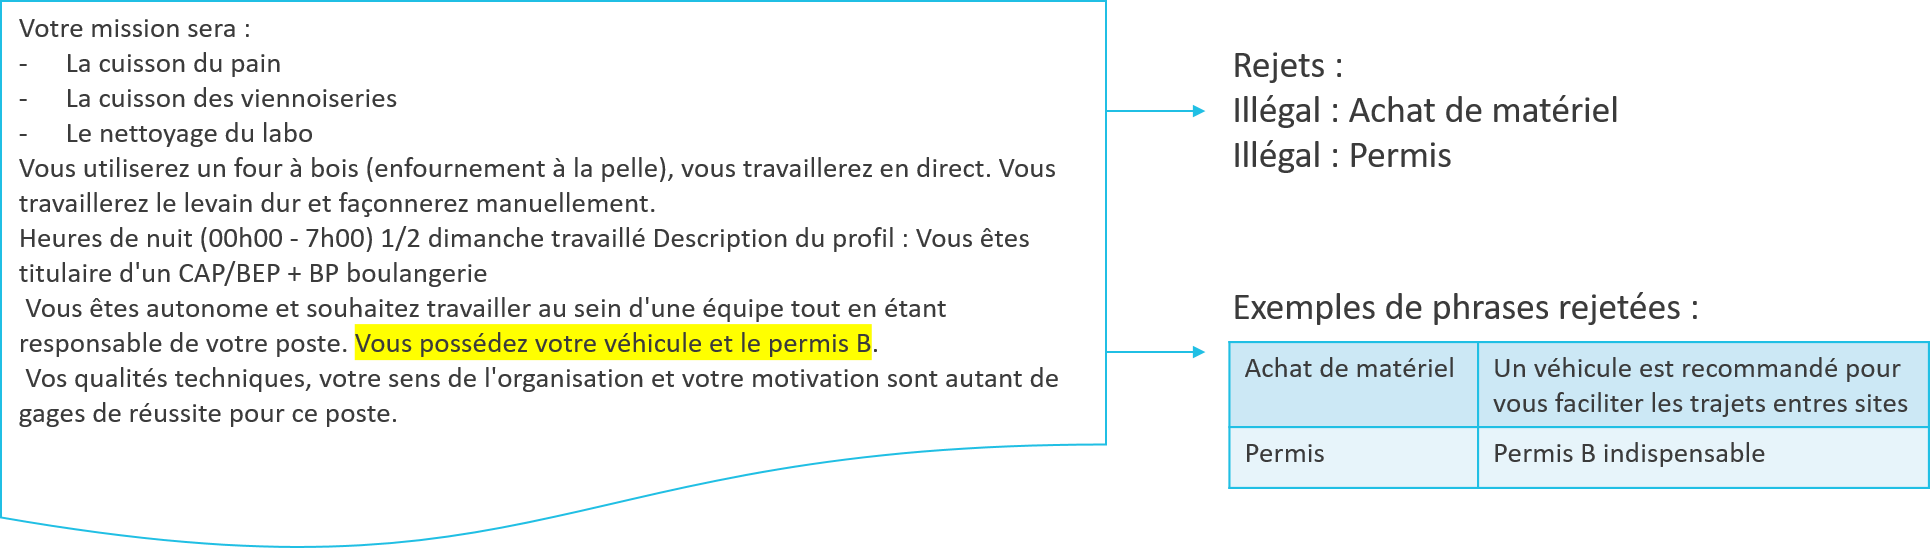
\includegraphics[width=\textwidth]{./S2-Explicabilite_locale/figures/prototype_exemple.png}
     \caption{Illustration d'explication par l'exemple}
     \label{fig:prototype_exemple}
 \end{figure}

\paragraph{Illustration d'un contre-exemple}
 % Quoi
 Enfin, la dernière maquette que nous proposons est l'explication par le contre-exemple, affichant pour chaque phrase rejetée une phrase proche, mais cette fois qui n'est pas rejetée par le système.
 % Pourquoi
 Ce type d'explication permet à l'utilisateur d'avoir un exemple de phrase acceptée, tout en étant proche sémantiquement de la phrase entraînant un rejet. Les contre-exemples sont illustrés en figure~\ref{fig:prototype_contre_exemple} avec comme précédemment une phrase par motif de rejet détecté.
 % illustration
 \begin{figure}[htpb!]
     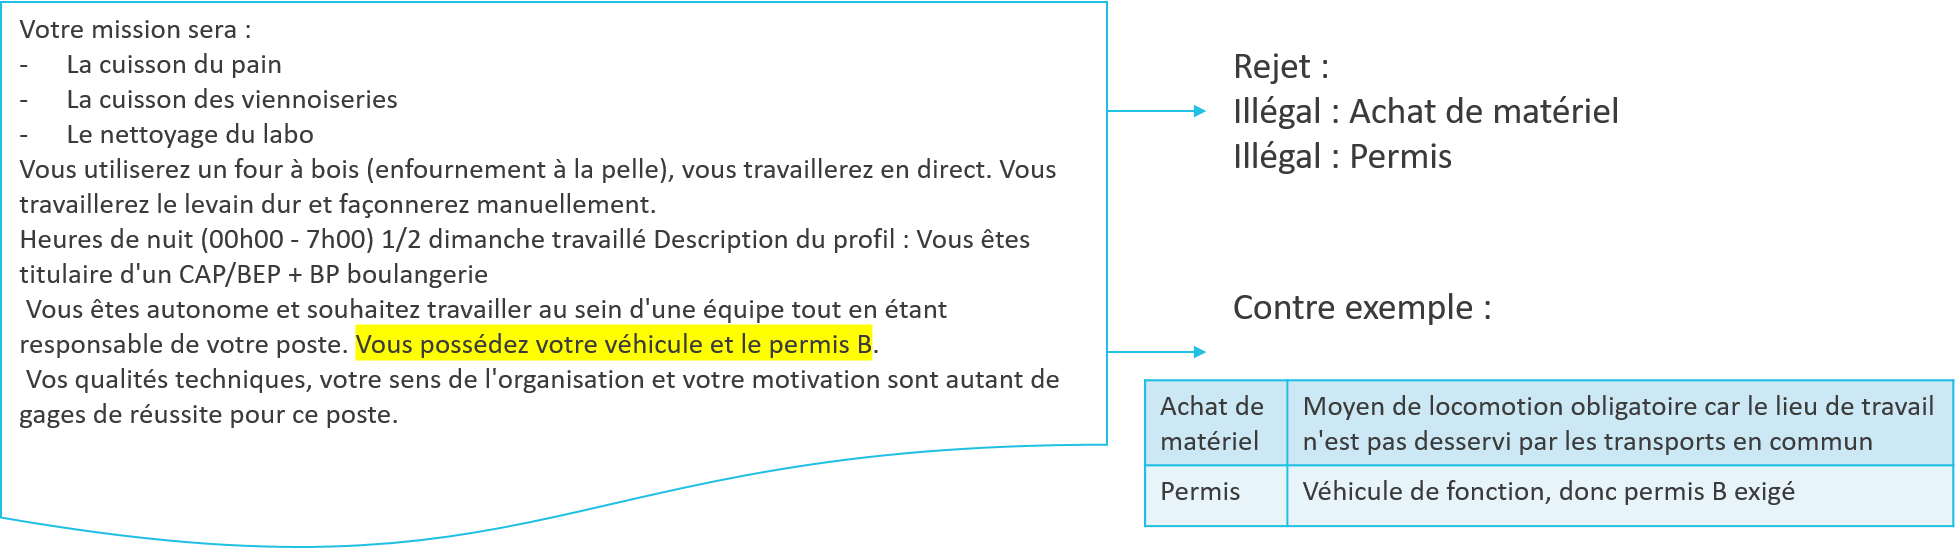
\includegraphics[width=\textwidth]{./S2-Explicabilite_locale/figures/prototype_contre_exemple.png}
     \caption{Illustration d'explication par le contre-exemple}
     \label{fig:prototype_contre_exemple}
 \end{figure}

Toutes ces illustrations sont présentées aux personnes participant au test d'utilisabilité, présenté dans le chapitre suivant.

\section{Conclusion}

% Objectif du chapitre
Dans ce chapitre, nous avons présenté le contexte applicatif de nos travaux, et les pré-requis à la réalisation de ceux-ci. Le cas d'usage illustrant nos travaux est développé en section~\ref{C2:usecase}. Nous avons généré des explications en section~\ref{C2:explications}, et préparé diverses illustrations section~\ref{C2:demonstrateur}.

% on en retire quoi, limites
La labellisation manuelle des données a mis en évidence des problématiques liées à la nature des données, avec la question de la prise en compte des mots vides de sens. La recherche d'une explication idéale qui corresponde aux préférences des utilisateurs est cruciale. Elle passe par la concertation des experts, mais également un travail de terrain coûteux de collecte d'une quantité significative d'explications, permettant d'obtenir un consensus.

Le temps limité de la thèse a amené à la labellisation d'une quantité restreinte de données. L'expérience ainsi acquise pointe vers la nécessité d'une définition collégiale des explications de référence. Avec une telle définition, il devient intéressant de collecter une quantité importante d'explications.

% Et la suite ?
Nous avons généré des explications, collecté des préférences et déterminé des explications faisant office de référence. Dans le prochain chapitre nous allons déterminer comment comparer des méthodes d'explicabilité, sur la forme et le fond.

\boitemagique{Résumé}{
\begin{itemize}
    \item[\checkmark] Nous avons labellisé un ensemble de données de test
    \item[\checkmark] La définition d'une explication de référence de qualité n'est pas une évidence
    \item[\checkmark] Nous avons généré des explications par mots importants
    \item[\checkmark] Nous avons proposé différentes visualisation d'explications locales
\end{itemize}
}
